\chapter[Introduction]{Introduction}
\section{Motivation}
Humankind has only a few ways to generate reliable, nonintermittent 
base load power: fossil fuels, hydro-power, geothermal power, and 
nuclear energy. Because of increasing global warming and climate 
change concerns, sources with negligible CO$_2$ footprints 
are crucial measures for global temperature change control. 
From an environmental viewpoint, hydro and nuclear power are 
preferable ways to generate reliable power. Nevertheless, the 
potential for a hydro-power is strictly limited by local geographical 
conditions, hence, the only option left is nuclear power. Nuclear 
power plants generate 4.9\% of global energy \cite{noauthor_key_2017}. 
Moreover, a nuclear share in energy generation is projected to stay 
constant through 2040 while electricity demand will 
increase by 30\% \cite{noauthor_world_2017}. Unfortunately, a negative 
public attitude to nuclear was formed in many developed countries 
because of concerns regarding safety, nuclear weapons 
proliferation, radioactive waste treatment, and competitiveness with 
other sources of energy (i.e. renewables). This negative public 
attitude to nuclear energy makes it challenging to justify its zero 
emissions benefits.

Generation IV International Forum (GIF) chose \glspl{MSR} among the 
six advanced reactor concepts for further research and development. 
\glspl{MSR} 
offer significant improvements ``in the four broad areas of 
sustainability, economics, safety and reliability, and proliferation 
resistance and physical protection" \cite{doe_technology_2002}. To 
achieve the goals formulated by the GIF, \glspl{MSR} 
simplify the reactor core and improve inherent safety by using 
liquid coolant which is also a fuel\footnote{Herein \glspl{MSR} are 
assumed to be reactors with liquid fuel which simultaneously serves 
as coolant.}. In a thermal spectrum \gls{MSR}, liquid fuel is consists 
of carrier salt (i.e. LiF or LiF-BeF$_2$) and fluorides of fissile 
and/or fertile materials (i.e. UF$_4$, PuF$_3$ and/or ThF$_4$) 
which is circulates in a loop-type primary circuit 
\cite{haubenreich_experience_1970}. 
This innovation leads to immediate advantages over traditional, 
solid-fueled, reactors. These include near-atmospheric pressure 
in the primary loop, relatively high coolant temperature, outstanding 
neutron economy, a high level of inherent safety, reduced fuel 
preprocessing, the ability to continuously remove fission products 
and add fissile and/or fertile elements without shutdown 
\cite{leblanc_molten_2010}. The possibility of continuously removing 
neutron poisons increases the potential fuel burnup and thus 
improves the resource utilization of \glspl{MSR}. Finally, the \gls{MSR} 
also could be employed for transmutation of 
spent fuel from current \glspl{LWR} \cite{fratoni_design_2004}.

Recently, interest in \glspl{MSR} has resurged, with multiple new companies 
pursuing commercialization of \gls{MSR} designs\footnote{Examples 
include liquid-fueled molten salt designs from Terrapower, Terrestrial, 
ThorCon, Flibe, Copenhagen Atomics, Elysium, etc.}. China's \gls{MSR} program 
was initiated in 2011 and promises to startup a 2MW$_{th}$ 
liquid-fueled test \gls{MSR} in 2020, a 10MW$_{th}$ 
demonstration reactor in 2025, and a gigawatt-level 
commercial reactor in 2050 \cite{zhang_review_2018}. The European 
Union funds the Safety Assessment of the Molten Salt Fast Reactor 
(SAMOFAR) project, in which several European research institutes and 
universities are developing various molten salt reactor prototypes 
such as the \gls{MSFR} \cite{fiorina_molten_2013} and the \gls{MOSART} 
\cite{ignatiev_molten_2014}.
To advance these \gls{MSR} concepts, particularly with respect 
to their strategies for online reprocessing and refueling, 
computational analysis methods capturing their unique reactor physics 
and process chemistry are needed. To correctly determine properties and 
operation conditions of \glspl{MSR}, including injection/removal schemes, 
computational tools to accurately model the processes which are unique for 
this particular reactor type. 

The main objective of the proposed work is to develop the online 
reprocessing simulation package, SaltProc, which couples with the 
continuous-energy Monte Carlo depletion calculation code, Serpent 2 
\cite{leppanen_serpent_2015}, for liquid-fueled \gls{MSR} depletion 
simulations. The ultimate objective of this effort is to develop a generic 
open-source tool capable of simulating a wide range of liquid-fueled 
systems, including two-fluid, multi-region designs, and validate it against 
existing modeling efforts. 

This document outlines the motivation, preliminary work, and future work 
proposed towards developing a simulation tool for analyzing fuel depletion in 
a liquid-fueled \glspl{MSR}. Chapter 1 serves as a literature review, 
providing background on fuel burnup, online fuel reprocessing approaches, 
safety parameters evolution during the reactor operation, and how these 
concepts have been applied to a wide range of \glspl{MSR} in the literature. 
Chapter 2 covers modeling online reprocessing details, including proposed 
software architecture, \gls{VV} method, demonstration cases, safety 
parameters evolution, and preliminary results. Specifically, these 
demonstration and verification efforts will 
focus on the \gls{TAP} \gls{MSR} because it well analyzed in the literature. 
Finally, Chapter 3 summarizes the conclusions reached concerning the 
appropriate mechanical and chemical models of fuel processing 
components to utilize in the online reprocessing plant simulation. 
Additionally, Chapter 3 outlines simulations plan for analyzing operational 
and safety characteristics evolution during \gls{TAP} reactor lifetime. 
Finally, remaining future work and expected contributions to the 
nuclear community will be summarized.

\section{Fuel burnup and online reprocessing}
All liquid-fueled \gls{MSR} designs involve varying levels of online fuel 
processing. Minimally, volatile gaseous fission products (e.g., Kr, Xe) 
escape from the fuel salt during routine reactor operation and must be 
captured. Additional systems might be used to enhance the removal of those 
elements. Most designs also call for the removal of rare earth metals from 
the core since these metals act as neutron poisons. Some designs suggest a 
more elaborate list of elements to process (figure~\ref{fig:periodic_tab}), 
including the temporary removal of protactinium from the salt or other 
regulation of the actinide inventory in the fuel salt 
\cite{ahmad_neutronics_2015}. Fresh fuel salt with dissolved fissile and/or 
fertile material (e.g., $^{233}$U, $^{232}$Th, \gls{LEU}, a transuranic 
vector from \gls{LWR} \gls{SNF}) make-up the salt mass loss caused by poisons 
removal and conserves the total mass in the primary loop.
\begin{figure}[htp!] % replace 't' with 'b' to 
  \centering
  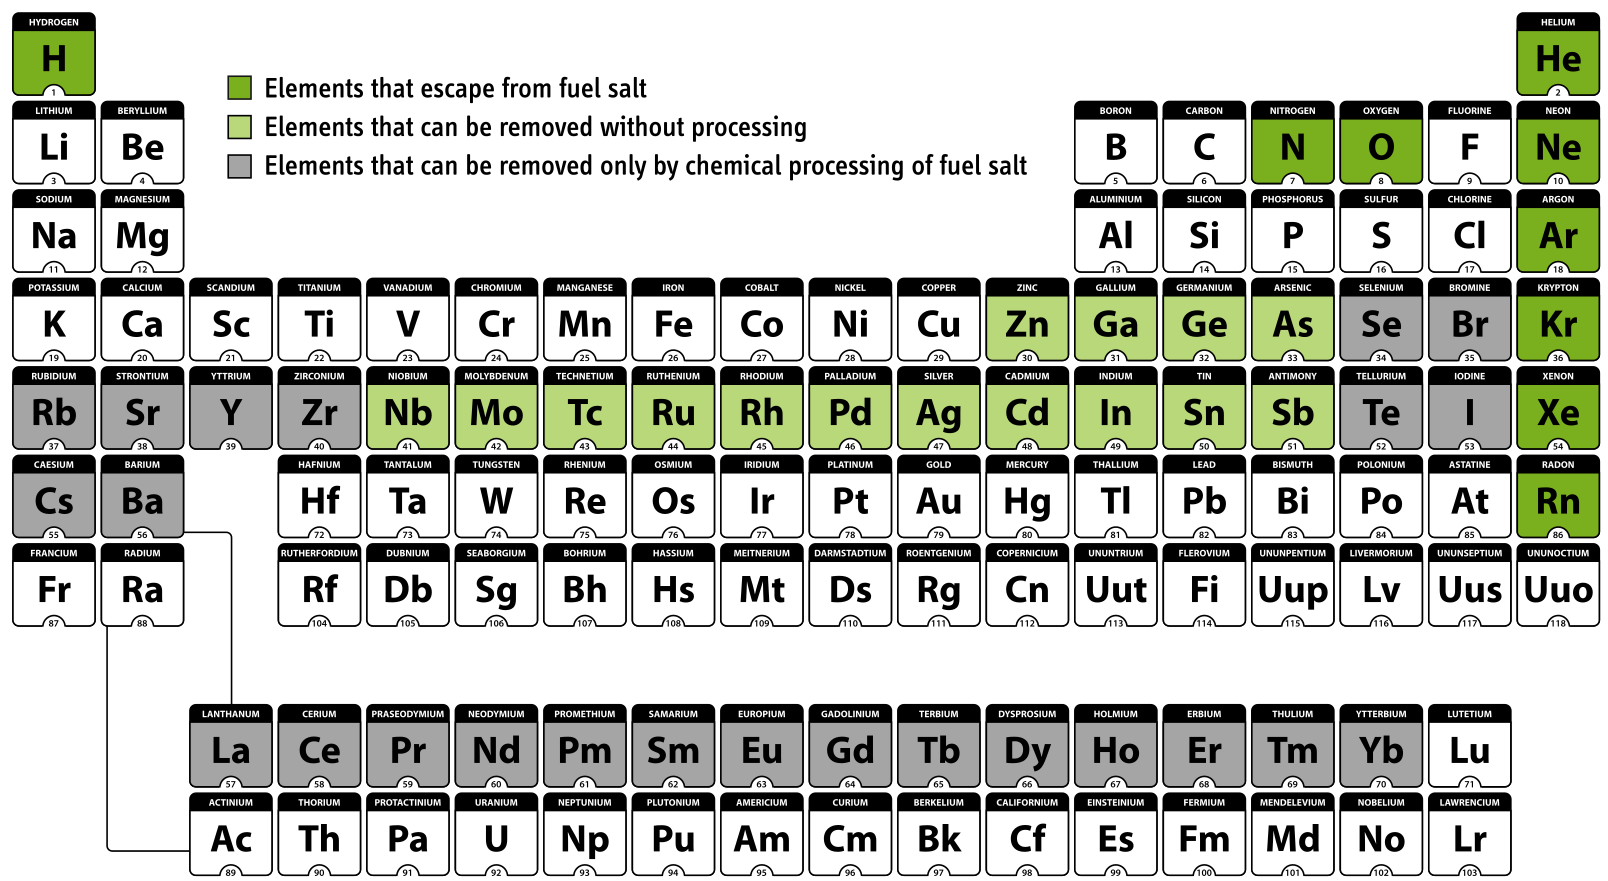
\includegraphics[width=0.9\textwidth]{periodic_map.png}
  \caption{Processing options for \gls{MSR} fuels (figure reproduced from 
  Ahmed \emph{et al.} \cite{ahmad_neutronics_2015}).}
  \label{fig:periodic_tab}
\end{figure}

Most of the liquid-fueled nuclear reactors adopted nonintermittent 
separations and feeds: the core material is moved to or from the core at all 
times (continuous) or specific intervals (batch). Contrarily, in a 
solid-fueled reactor, fission products and actinides 
remain within the initial fuel material during and after operation until 
reprocessing. The ability to perform online fuel salt reprocessing improves 
the potential neutronic performance of liquid-fueled reactors. First, it 
is unnecessary for liquid-fueled reactors to operate with excess reactivity 
because fissile material is continuously being added to the core. Second, 
continuously removing fission products, including strong absorbers (poisons) 
should significantly improve fuel utilization and decrease parasitic 
neutron absorption. Finally, for a breeder (reactor with a 
\gls{CR}\footnote{\gls{CR} $\equiv$ fissile generated/fissile consumed: if CR 
$<$ 1, the reactor is a ``converter''; CR $\equiv$ 1, an ``isobreeder''; 
CR $>$ 1, a ``breeder.''}$>1$, excess of fissile material might be 
continuously evacuated from the core and used to startup new reactors. 
Nevertheless, the removal of each element from the liquid fuel salt presents 
a unique challenge in terms of chemical separation, storage, and disposal of 
the separated materials.

Continuous fuel salt reprocessing prevents the usage of most contemporary 
nuclear reactor fuel burnup software. Few code packages were developed 
specifically for \gls{MSR} depletion simulations at universities and research 
institutions and not available for external use. The foundation for these 
in-house tools was based on early \gls{MSR} simulation methods at \gls{ORNL}, 
which integrated neutronic and fuel cycle codes (i.e., Reactor Optimum Design 
(ROD) \cite{bauman_rod_1971}) into operational plant tools (i.e., Multiregion 
Processing Plant (MRPP) \cite{kee_mrpp_1976}) for \gls{MSR} and reprocessing 
system design. More recently, Nuttin \emph{et al.} developed in-house 
depletion code REM which directly couples with the \gls{MCNP}  
\cite{noauthor_mcnp_2004} to simulate fuel salt material evolution in 
simplified \gls{MSBR}-like reactor. That work directly integrated
Bateman differential equations using neutron flux from the \gls{MCNP}, 
tracking all the isotopes available in the data library, and control 
reactivity to maintain reactor critical.

A summary of recent efforts is listed in table~\ref{tab:msr_codes}.